\documentclass[tikz,a4paper]{standalone}
\usetikzlibrary{shadings}
\usepackage{pgfplots}
\usepackage{tikz,tikz-3dplot}
\usepackage{amsmath,amsthm}
\usepackage{amssymb}
\usepackage{amsfonts}
\usepackage{times}


\usetikzlibrary{positioning,arrows.meta,quotes}
\usetikzlibrary{shapes,snakes}
\usetikzlibrary{bayesnet}
\tikzset{>=latex}

\begin{document}
\pgfdeclarelayer{back}
\pgfdeclarelayer{fore}
\pgfdeclarelayer{foreback}
\pgfsetlayers{back,foreback,main,fore}
\definecolor{back}{RGB}{20,91,147}
\definecolor{back1}{RGB}{29,100,114}
\definecolor{left1}{RGB}{43,60,67}
\definecolor{right1}{RGB}{240,240,215}
\definecolor{bottom}{RGB}{8,77,182}
\definecolor{axback}{RGB}{186,163,204}
\definecolor{colorB}{RGB}{78,201,176}
\definecolor{colorC}{RGB}{11,127,110}
\definecolor{colorD}{RGB}{23,79,114}

\begin{tikzpicture}
\node[minimum width=21.587cm,minimum height=27.937cm,inner sep=0pt,outer sep=0pt](box){};

\begin{pgfonlayer}{back}
\node[scale=1.6,opacity=1] at (0,0) {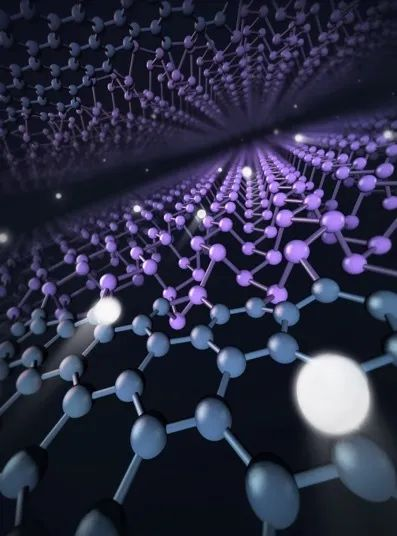
\includegraphics{fig75}};
\end{pgfonlayer}

%\begin{pgfonlayer}{back}
%\shade[outer color=back,inner color=back](-10.9935,-15.5) rectangle (10.9935,15.5);
%\end{pgfonlayer}

%\filldraw[fill=violet,draw=violet,rotate=10] (0,6.5) -- (-8,-3.5) arc (240:290:20cm) --(0,6.5);
%\filldraw[fill=back,draw=back,rotate=10] (0,10.5) -- (-8,-3) arc (240:285:23cm) --(0,10.5);
%
%\filldraw[fill=orange,draw=orange] (0,7) -- (-8,-3) arc (240:290:20cm) --(0,7);
%\filldraw[fill=back,draw=back] (0,11) -- (-8,-2.5) arc (240:285:23cm) --(0,11);

\draw[draw=red!60!yellow,fill=orange](4.3,0)circle (1.8cm);
\draw[draw=blue,fill=blue](4.3,0)circle (2pt);
\node[blue,below] at(4.2,0){$\varphi (p)$};
%\useasboundingbox[dashed,very thin,draw=white](2,-2.5)grid(7,2.5);
\node[scale=1.2] at (-3.8,0.2) {
\begin{tikzpicture}
\pgfplotsset{
/pgfplots/colormap={jet}{rgb255(0cm)=(0,0,128) rgb255(1cm)=(0,0,255)
rgb255(3cm)=(0,255,255) rgb255(5cm)=(255,255,0) rgb255(7cm)=(255,0,0) rgb255(8cm)=(128,0,0)}
}
\begin{axis}[
view={25}{30},
white,
minor tick num=4,
major tick length=1mm,
tick style={gray},
minor tick length=0mm,
%axis line shift=0pt,
%axis background/.style={
%shade,top color=axback,bottom color=axback,
%},
%grid,
%hide axis,
]
\addplot3[domain=-2:2,y domain=-2:2,samples=20,surf]{x^2-y^2};
\addplot3[domain=-1:1,y domain=-1:1,faceted color=magenta,samples=40,surf]{x^2-y^2};

\end{axis}
\end{tikzpicture}
};

\draw[blue!65!yellow,thick,<-](4.2,0.2) arc (50:130:6cm);
\draw[draw=blue,fill=blue](-3.5,-0.05)circle (2pt)node[below,blue]{$p$};
\node[blue,above] at(-6,1.3){$M$};
\node[blue,above] at(-4,-0.2){$U$};
\node[blue,above] at(5,0){$U'$};
\node[white,above,scale=3,opacity=0.6,xslant=0.4] at(0,-5.5){$\varphi: \mathbb{R}^{3}\rightarrow \mathbb{R}^{2}$};
\node[white,above,scale=2.5,opacity=1] at(0,-7){$(x,y,z)\mapsto (u(x,y,z),v(x,y,z))$};
\node[white,scale=2] at(0,7){\textit{Banach Spaces}};
\node[
scale=2,
orange,
%xshift=-0.3cm,
%left color=left1,
%right color=right1,
%xslant=0.8,
%yshift=0.4cm
] at(0,-12){http://www.latexstudio.net};
\node[scale=5,orange] at(0,10.5){\bfseries\rmfamily Awesome-drawing};
\node[white,above,scale=1.5] at(1,1.6){$\varphi$};
\node[scale=3,orange] at(0,8.5){\bfseries\rmfamily  By Using TikZ};

\end{tikzpicture}



\end{document} 